%!TeX encoding=utf8

\section{Bose Einstein Condensate}

\subsection{Questions}
\begin{itemize}
        \item $\int \frac{1}{r^{n}} \mathrm{d^{3}r}$ divergent just for $n \leq 3 $ ?
        \item What is an s-wave?
        \item if $l < \frac{n-3}{2}$,
        \item and like $k^{n-2}$ otherwise (Landau and Lishitz, 1977). For a van der
        Waals-like potential $(n = 6)$, only $l = 0$ (s-wave) matters at low energies. Whats with $l=0$? Lifschitz is a typo?
        \item In the notes: eq. 1.8 to 1.9 the commutator $[\psi, \psi^{\dagger}]$ was used, but from 1.9 to 1.10 Bogoliubov aproximation was used, why not directly on 1.8 ?
        \item What is the derivation of 1.11? Its a FFT, but what are the xact steps?
        \item What are the python packages to use operators like $\hat{\psi}$? There is some sympy implementation, but probably there is a better one?
        \item how to get from 1.11 to 1.12? Is it a commutator expansion? Why $q$ is disappearing?
        \item In 1.17 $\omega_{\rho}$ part has a factor 2, but $\omega_{z}$ not, despite beeing symmetric in $\psi$. Why?
        \item What is variable $a$? Why should $a > 0$ as repulsive short-range interactions stabilize the BEC (p.10)?
        \item ``When the atomic density grows due to the attractive interaction, three-body losses predominantly occur in the high-density region. '' What does three-body losses mean?
        \item ``As the collapse occurs mainly in the x-y direction due to anisotropy of the DDI (in the absence of inelastic losses, the condensate would indeed become an infinitely thin cigar-shaped cloud along z),
        and therefore the condensate explodes essentially radially, producing the anisotropic
        shape of the cloud.'' Why is the collaps not along z axis?
        \item How are the regions stable, metastable, unstable derived in Figure 1.5, here Figure \ref{fig:acrit}?
\end{itemize}

\begin{figure}[H]
    \centering
    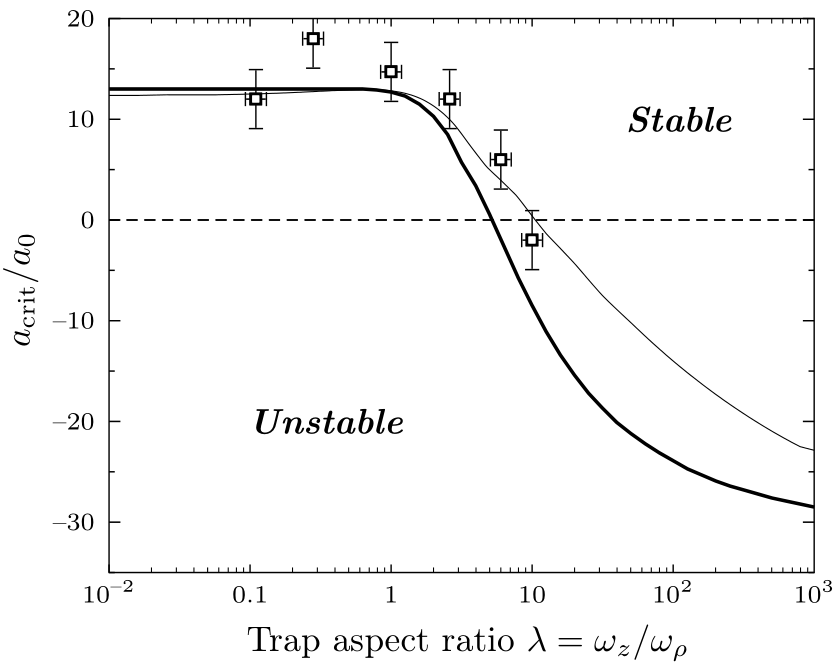
\includegraphics[width=0.7\textwidth]{IMAGE/acrit.png}\\
    \caption{Logo}
    \textsc{Santos}, \emph{title} (year)
    \label{fig:acrit}
\end{figure}

\begin{itemize}
        \item Typo in ``we obtain a 1D equation similar to the a GP equation'', just the or a
        \item ``ground-state wave-function is independent of the in-plane coordinates '' Why?
        \item 1.26 to 1.27, where does the $U_{dd}$ go?
        \item Typo If: ``roton momentum. if this were so''
        \item Why should a modulation with a finite wavelength allow superfluids?
        \item Typo repeatance: ``the width of the width''
        \item What are the spin-F matrizes?
        \item Is the occurance of these spin textures in Figure \ref{fig:helical} special?
\end{itemize}

\begin{figure}[H]
    \centering
    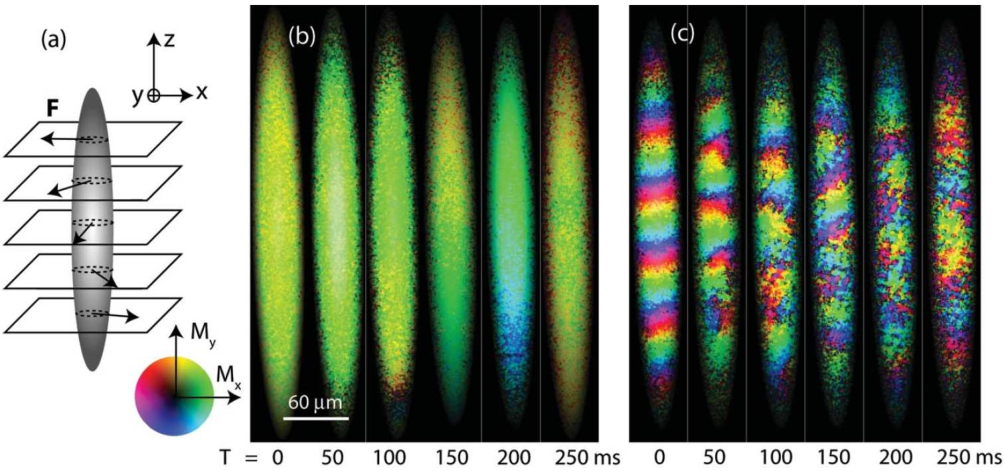
\includegraphics[width=0.7\textwidth]{IMAGE/helical.png}\\
    \caption{Is the occurance of these textures special?}
    \textsc{Santos}, \emph{title} (year)
    \label{fig:helical}
\end{figure}

\subsection{Summary}
\begin{itemize}
        \item dipol-dipol interaction (DDI): \begin{equation}
          U(r) = \underbrace{g \delta (r)}_{\frac{4 \pi \hbar^{2} a(d) \delta(r)}{m}} + \underbrace{U_{dd}(r)}_{\frac{C_{dd}}{4 \pi} \frac{(e_{1} \cdot e_{2}) r^{2} - 3(e_{1} \cdot r) (e_{2} \cdot r)}{r^{5}}}
        \end{equation}
        \item Use pseudo potential as dipol-dipol interaction is anisotropic and all partial wave (different l) mix
        \item coupling of different channels generates short-range contribution in the s-channel $s=0$ $\Rightarrow$ by changing DDI strength $a$ gets modified too $\Rightarrow$ shape resonances $\Rightarrow$ virtual state transform into a new ground state
        \item for fermions s-channel does not exists, so just long-range
        \item FFT of $U_{dd}$ using sperical harmonics $Y_{lm}$ gives:
        \begin{equation}
          \tilde{U_{dd}}(k) = \int \mathrm{d^{r} r} U_{dd}(r) e^{-ik \cdot r}= \frac{C_{dd}}{3}\left(3 \cos^{2}(\theta_{k}) - 1 \right)
        \end{equation}
        \item Use DDI in Gross-Pitajevski Equation, FFT, approximate to 2nd order, diagonalize with Bogoliubov transform
        \item As a result the square root can be imaginary, so the BEC gets dynamically unstable for long-wave length (phonon-instability):
            \begin{align}
              \epsilon(p) &= \sqrt{\frac{p^{2}}{2m} \left[\frac{p^{2}}{2m} + 2 n_{0} \left( g + \tilde{U_{dd}(p)} \right)\right]} \\
              &= p c_{s} \sqrt{1 + \epsilon_{dd} \left( 3 \cos^{2} \theta_{p} - 1 \right)} \\
              &\underset{p \rightarrow 0}{=} p c_{s} \sqrt{1 - \epsilon_{dd}}
            \end{align}
        \item For dipolar BEC the trap geometry is crucial (for non-dipolar not)
        \item ``pancake traps'' can stabilize the phonon-instability
        \item qualitative features for $a_{crit}(\lambda)$ by gaussian ansatz, for exact numerical solution non-local Gross-Pitaevskii Equation needed
\end{itemize}

\begin{figure}[H]
    \centering
    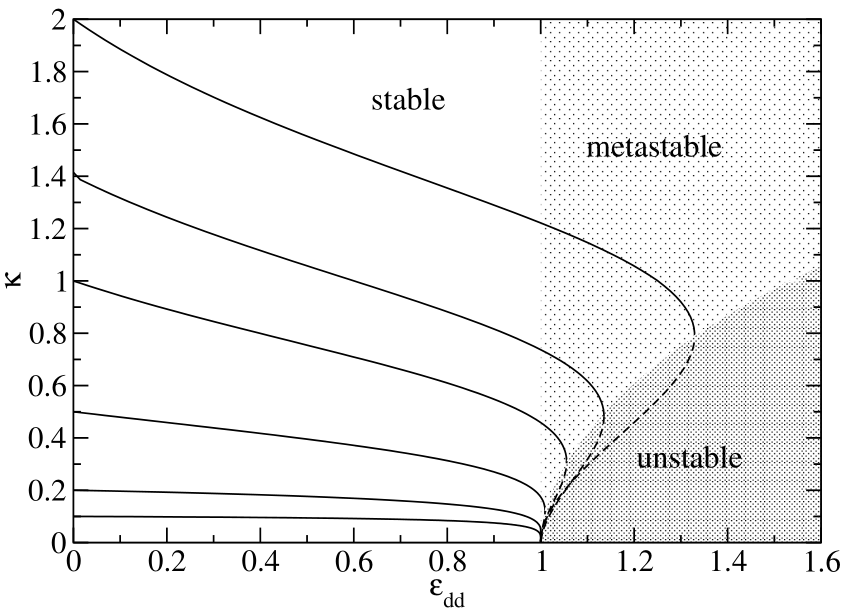
\includegraphics[width=0.7\textwidth]{IMAGE/stability.png}\\
    \caption{Logo}
    \textsc{Santos}, \emph{title} (year)
    \label{fig:stability}
\end{figure}

\begin{itemize}
        \item for sufficiently strong interactions, we may neglect quantum pressure, and consider the Thomas-Fermi (TF) regime
        \item TF solution for the trapped BEC has the same inverted parabola shape (as in non-dipolar case)
        \item BEC is prolat for $0 < \kappa < 1$ and $1 < \kappa$ oblat
        \item Bogoliubov-de Gennes Equation shows that the nonlocal character of the DDI causes a momentum dependend coupling constant, leading to a roton-like dispersion law, leading to dynamically instability, when the roton $\beta = \frac{g_{d}}{g}$ touches zero (experimetally not obeserved yet)
        \item by varying the density, the frequency of the confinement, and the short-range coupling,
        one can control the spectrum (roton minimum deeper/shallower)
        \item sequence of the non-local non-linearity 2D bright solitary waves may become stable
under appropriate conditions (Pedri and Santos, 2005)
        \item two instability regions for 2D solitons (against col-
        lapse and against unlimited expansion)
  \item $\tilde{g}_{cr}(\beta) \equiv \frac{g N_{cr}}{2 \pi l_{z}}$, so stable 2D anisotropic self-localised solitons exists just for $N < N_{cr}$
        \item non-dipolar BECs scatter elastically, the scattering of dipolar solitons is inelastic due to the lack integrability
        \item The solitons may transfer centre-of-mass energy into internal vibrational modes,
        resulting in intriguing scattering properties:

        \begin{itemize}
          \item including soliton fusion (Fig. 1.8)
          \item appearance of strong inelastic resonances
          \item possibility of observing 2D- soliton spiraling as that already observed in photo-refractive materials
        \end{itemize}

        \item Dipolar effects in spinor condensates
        \begin{itemize}
            \item spinor BECs: we focus on an effect which resembles the Einstein-de Haas effect
            \item Because of Zeeman sub-levels short-range interactions may occur in different s-wave scattering channels with different total angular momentum (for bosons even number) ( spin-1 bosons we have just F = 0 and F = 2)
            \item Each scattering channel has an associated s-wave scattering length $a_{F}$
            \item short-range interactions necessarily preserve the spin projection Sz
            \item DDI does not necessarily conserve the spin projection along the quantisation axis as DDI is anisotropic
            \item for initially maximally stretched state ($m_{F} =  - F$)
            \item short-range interactions cannot induce any spinor dynamics (due to conservation of total magnetisation $S_{z}$
            \item DDI may induce a transfer to $m_{F} + 1$
            \item for cylindrical symmetry around the quantisation axis, this violation of the spin projection is accompanied by a transfer of angular momentum to the centre of mass, resembling the well known Einstein-de Haas effect $\Rightarrow$ initially spin-polarised dipolar condensate can generate dynamically vorticity
            \item Einstein-de Haas effect is destroyed by weak magnetic fields (1 mG)
            \item the dominant Larmor precession, and invoking rotating-wave-approximation arguments, the physics must be constrained to manifolds of preserved magnetisation (2D optical lattices could help)
            \item Effect of DDI could be even observable under conserved $S_{z}$ (alkali spinor condensates)
            \item spin-changing collisions: collisions that conserve $S_{z}$, but do not conserve the relative population of the different Zeeman components
            \item Spin-changing collisions are characterised by an energy scale proportional
to the difference between scattering lengths at different channels
            \item this difference is very small, so can be significantly modified by the presence of other small energy scales (DDI) $\Rightarrow$ helical spin textures
        \end{itemize}
\end{itemize}

\begin{figure}[H]
    \centering
    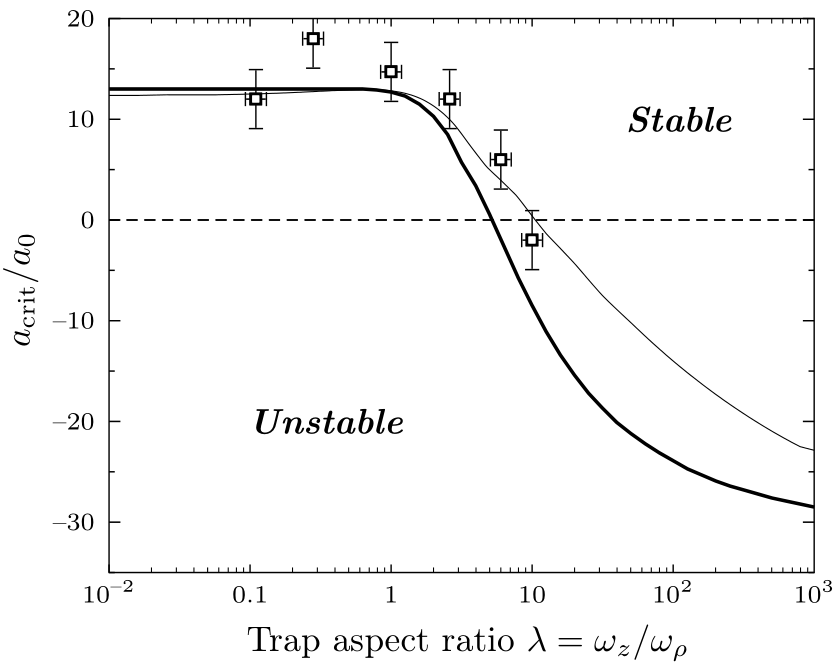
\includegraphics[width=0.7\textwidth]{IMAGE/acrit.png}\\
    \caption{Logo}
    \textsc{Santos}, \emph{title} (year)
    \label{fig:acrit}
\end{figure}

\begin{itemize}
        \item Typo in ``we obtain a 1D equation similar to the a GP equation'', just the or a
        \item ``ground-state wave-function is independent of the in-plane coordinates '' Why?
        \item 1.26 to 1.27, where does the $U_{dd}$ go?
        \item Typo If: ``roton momentum. if this were so''
        \item Why should a modulation with a finite wavelength allow superfluids?
        \item Typo repeatance: ``the width of the width''
        \item What are the spin-F matrizes?
        \item Is the occurance of these spin textures in Figure \ref{fig:helical} special?
\end{itemize}

\section{Supersolids}

\begin{itemize}
    \item supersolid: features both the crystalline structure of a solid and the frictionless flow of a superfluid
In this state, every constituent atom is part of the solid and the superfluid simultaneously
    \item direct observation was limited to systems where the structure formation was mediated by external light fields
    \item beyond mean-field approximation leads to corrections to the ground
state energy stemming from quantum fluctuations of the collective modes in a BEC (LHY-correction)
    \item In 2018 quantum droplets in a Bose-Bose mixture were observed
    \item mean- field energy depends on the difference of the two coupling constants $\delta(g) = |g_{rep}| - |g_{att}|$ \item LHY-correction depends on the individual coupling constants
    \item For weakly attractive combination of interactions, a repulsive beyond mean-field correction can stabilize the BEC
    \item after a peak density increasing the number of particles only leads to an increase in the
size of the droplet
    \item eGPE: kinetic energy, external trapping, and two-body interactions, LHY
    \item beyond mean-field correction has only been calculated for a homogeneous system and can therefore only be included within a local-density approximation
    \item QMC calculations in full many-body system verified the formation
    \item intra-species scattering lengths $a_{11}$ and $a_{22}$ lead to different equilibrium densities $n^{(i)}_{0}$ for the two components of the mixture.
    \item droplet forms an intrinsic imbalance in the atom numbers of the two components ($\frac{N1}{N2} = \sqrt{\frac{a_{22}}{a_{11}}}$ )
    \item larger density than in original BEC increases the rate of three-body loss $\Rightarrow$ extra term in eGPE
\end{itemize}

\begin{figure}[H]
    \centering
    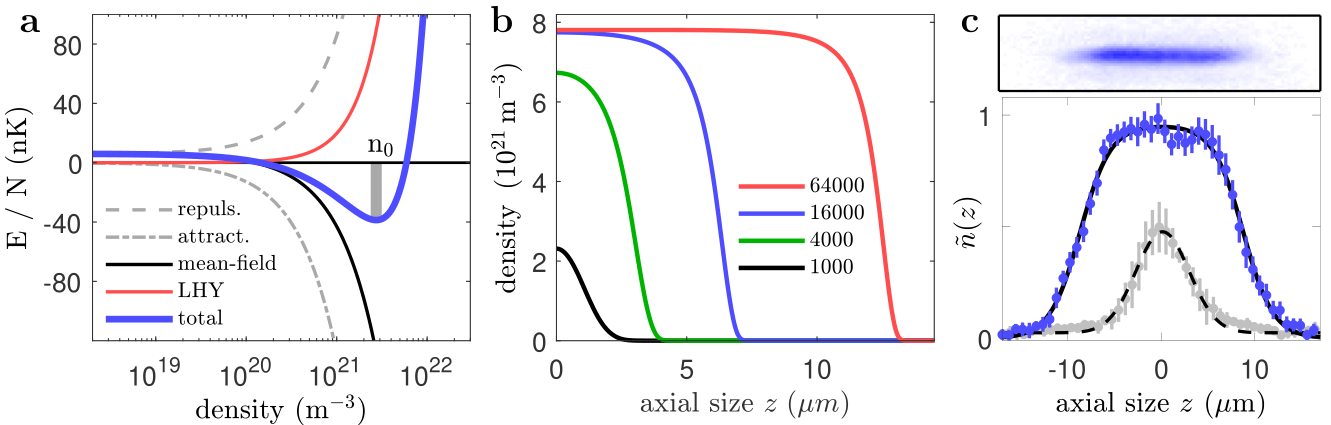
\includegraphics[width=0.7\textwidth]{IMAGE/droplet.png}\\
    \caption{Peak density of the droplet saturates in z-driection}
    \textsc{Santos}, \emph{title} (year)
    \label{fig:droplet}
\end{figure}
